\subsection{Neural Networks}\label{sec:NN}
\ac{NN} have been an idea for more than 80 years and are today one of the 
most popular and successful \ac{ML} methods. The key to its popularity stems from
its versatility, achieving high performance in a large range of both regression 
and classification problems. One of the defining qualities in a \ac{NN} is the 
possibility of diverse architecture, meaning that a there are many
categorize of \ac{NN}, where each category has an even deeper selection of
networks. Categories ranging from \ac{CNN}, \ac{RNN} to simple \ac{FFNN}, where each
category is specified for their own set of problems. In this section I will introduce 
some fundamental definitions in regard to \ac{NN}, as well go through the underlying 
algorithm of the back- and forward propagation.

\subsubsection*{General structure}
There are often drawn comparisons between the structure of the neural network, 
and the way the human mind operate, hence neural. Similarly to the human mind, a \ac{NN} is 
composed of different neurons communicating information backwards and forwards in different 
regions In the case of a neural network we call these regions layers. All layers
are composed of a specified number of neurons. A \ac{NN} has three types of layers;
\emph{input-layer}, \emph{hidden-layer} and \emph{output-layer}. There is only one input layer, and it has
the same number of nodes equal to the number of features for each data point. 
There can be an arbitrary number of hidden layers, with each hidden-layer containing
an arbitrary number of nodes. Finally, the \ac{NN} has an output layer. The output-layer
contains a number of nodes equal to the number of features for the target.
\\
The neural network functions by passing information in between the different layers though 
nodes. The nodes are simply pockets of information, each containing a value. 
All the nodes in the input layer are connected to all the nodes in the nearest hidden layer,
and likewise said hidden layer is connected to the next hidden layer. This structure continues
until we reach the final layer, the output layer. The structure is illustrated in figure
\ref{fig:NN}. The figure shows a simple \ac{NN} with a 2 dimensional data set (2 nodes in input-layer),
2 hidden layers with three nodes each and a 1 dimensional target value. It also illustrates 
how a \ac{NN} aims to map from data, $x_i$ to a prediction $y_i$.
\begin{figure}
    \centering
    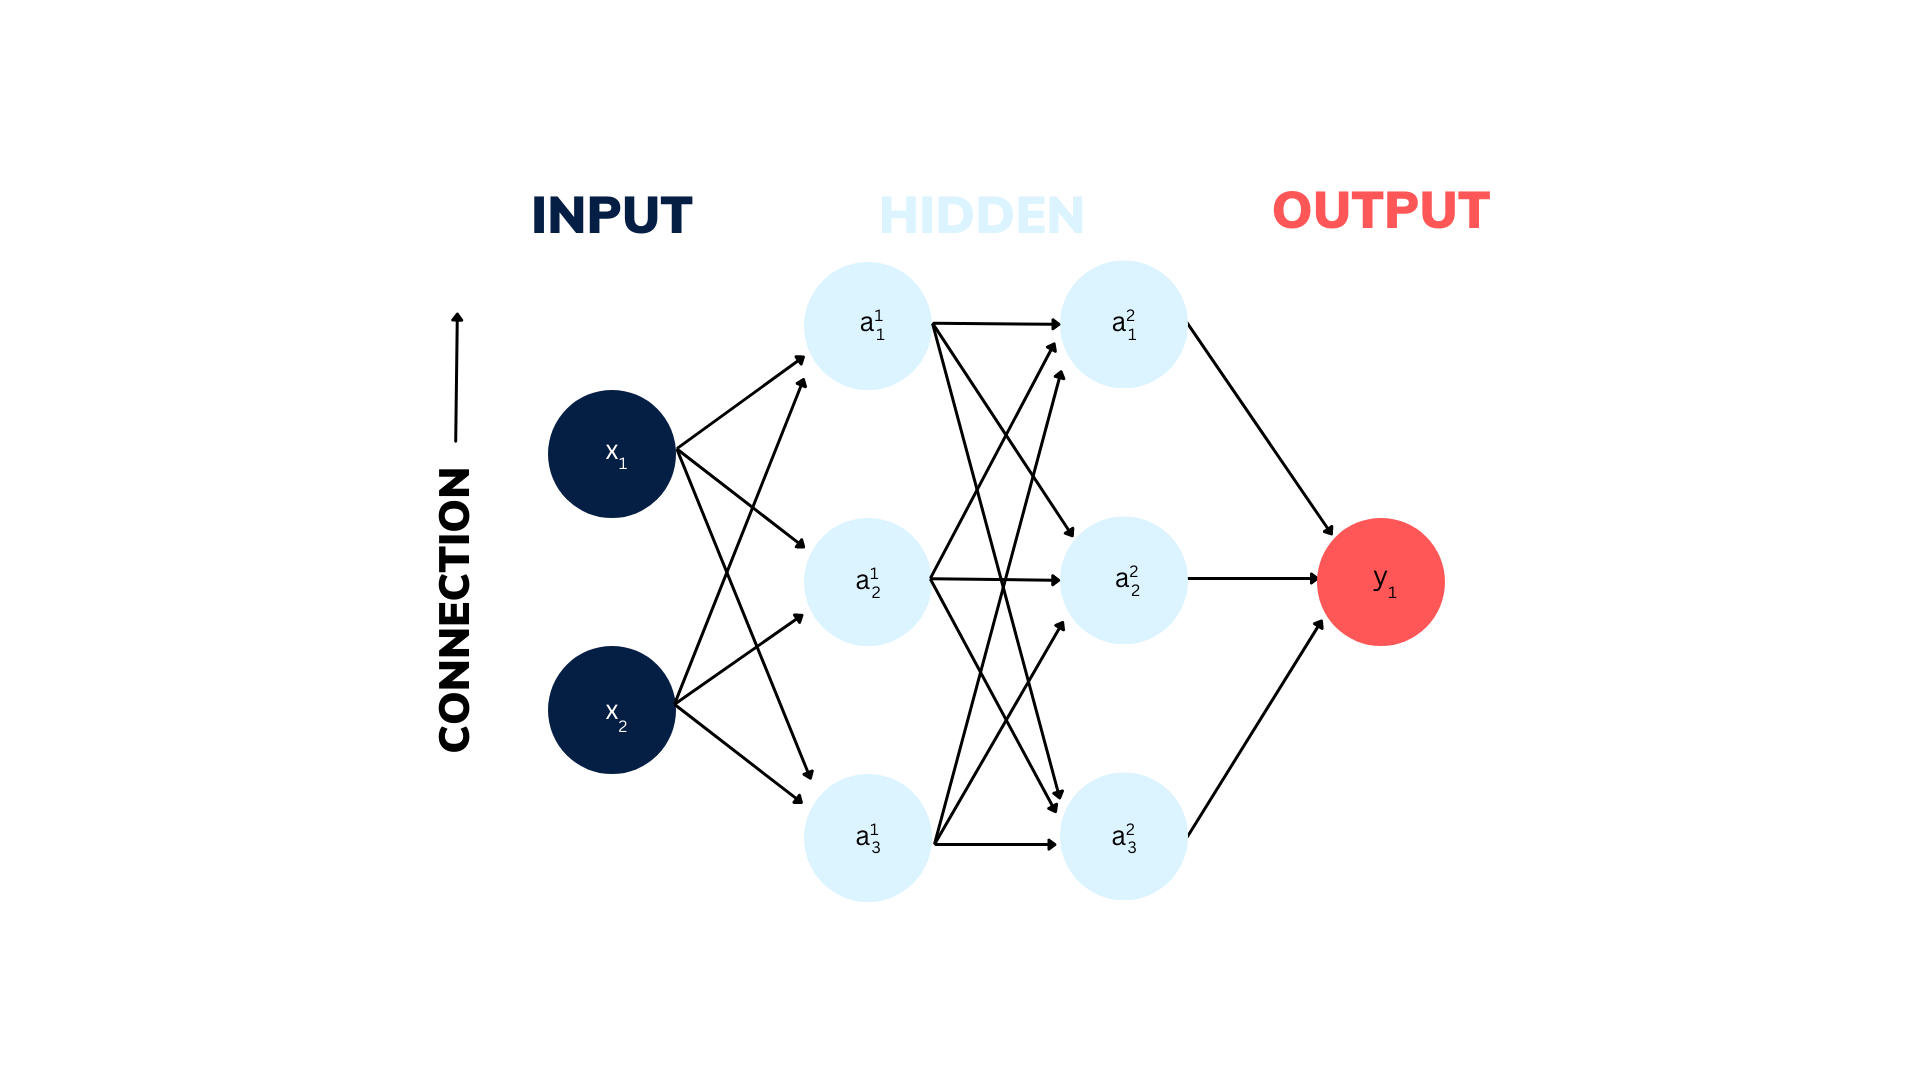
\includegraphics[width=0.9\textwidth]{Figures/Illustrations/Input_labels.png}
    \vspace*{-12.5mm} 
    \caption{An illustration of a \ac{NN} with two hidden layers.}
    \label{fig:NN}
\end{figure}
In figure \ref{fig:NN} we can see how all the different nodes are connected, illustrated by 
the arrows. The passing of values between different nodes are controlled by a set of weights and
bias parameters. These parameters are defined for each connection and are what will be tuned 
during training. The weights and biases for a given connection of two nodes, defines the effect on node 
has on the other.
\\
In a traditional \ac{FFNN} the information is passed linearly (in figure \ref{fig:NN}, from left to right) 
in a process we call \emph{forward-propogation}. Other variants can include the information taking a more 
complex route. It is often the route from input- to output-layer that categorizes the type of \ac{NN}. In 
this report I used a simple \ac{FFNN}. 

\subsubsection{Feeding Forward}\label{subsubsec:FP}
With the structure described in the previous section, a trained model, $\mathcal{F}$ produces a prediction,
$\bf{y}$ for a data set $\bf{x}$ by passing information from input-layer, through all hidden-layers then
to output-layer through forward-propagation. In this section I aim to explain the underlying math.
\\
We imagine the passing from hidden-layer l-1 to l, where $l \in \{0,1,...,N_L \}$ and $N_L$ is equal to the
number of hidden layers. The value of a node in layer l, is defined as $a^l_j$, where $j\in \{0,1,...,N^l\}$ and 
$N^l$ is equal to the number of nodes in l.


\subsubsection{Back Propagation}\label{subsubsec:FP}
